\documentclass[12pt, a4paper]{article}
\usepackage{../../../myconfig} % Gọi file cấu hình từ ngoài gốc vào
% ==========================================
% BẮT ĐẦU NỘI DUNG TÀI LIỆU
% ==========================================
\begin{document}

% Truyền 3 tham số: {Nhãn cam} {Chữ to chính giữa} {Chữ ở góc phải Header}
\titlebox{Chủ đề: Tích phân}{Tốc dộ thay đổi đại lượng và lượng tích lũy}{Thay đổi đại lượng}

% --- CÂU 1 ---
\questionShortAnswer{0}{1}{Người ta quan sát một quần thể vi khuẩn đang tăng trưởng, ban đầu gồm 500 vi khuẩn. Sau một ngày và sau bốn ngày kể từ khi bắt đầu quan sát, số lượng vi khuẩn của quần thể đó tương ứng là 600 vi khuẩn, 1300 vi khuẩn. Gọi \(P(t)\) là số lượng vi khuẩn của quần thể đó tại thời điểm \(t\) ngày kể từ khi bắt đầu quan sát, \(0 \leq t \leq 10\). Người ta ước tính tốc độ tăng trưởng của quần thể vi khuẩn đó được mô tả bởi \(P'(t) = at + b\sqrt{t}\) (vi khuẩn/ngày), trong đó \(a, b\) là hằng số. Hỏi số lượng vi khuẩn của quần thể đó sau 9 ngày kể từ khi bắt đầu quan sát là bao nhiêu?
}

% --- CÂU 2 ---
\questionShortAnswer{0}{2}{Tại một trại tôm ở một địa phương, do sự cố mất điện tạm thời, khi hệ thống hoạt động trở lại (\(t = 0\)), mực nước trong bể hình hộp chữ nhật (diện tích đáy \(S = 40\) m\(^2\)) đang ở mức 0,5 mét. Để bù đắp lượng oxy thiếu hụt, máy bơm hoạt động với công suất tăng cường theo thời gian: \(V_{vào} = 4t + 12\) (m\(^3\)/giờ). Hệ thống xả tự động vẫn vận hành theo công thức: \(V_{ra} = \dfrac{40h(t)}{t+2}\) (m\(^3\)/giờ) để đảm bảo áp suất đáy, với \(h(t)\) là chiều cao mực nước tại thời điểm \(t\) (tính bằng mét). Sau 2 giờ vận hành kể từ khi có điện lại, mực nước trong bể tăng bao nhiêu mét so với lúc ban đầu? (làm tròn kết quả đến hàng phần trăm).
\begin{figure}[H]
    \centering
    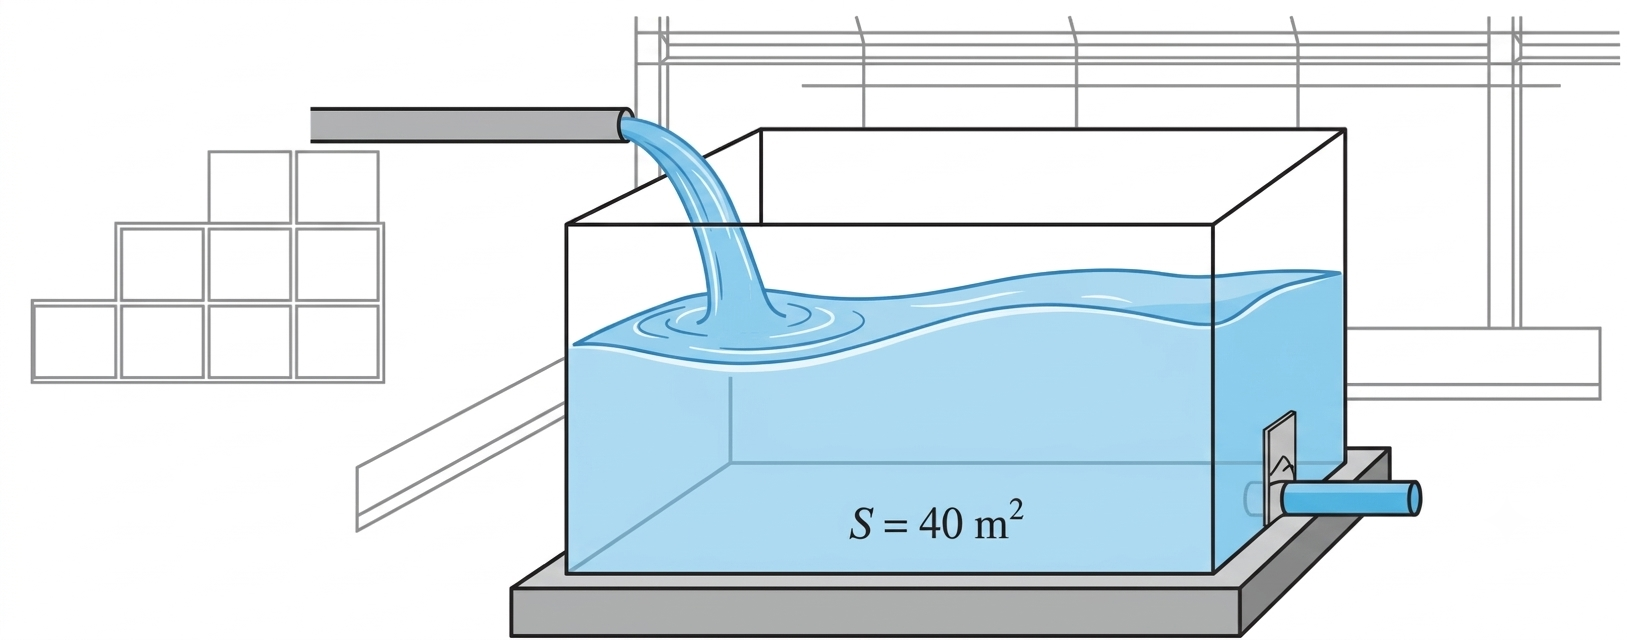
\includegraphics[width=0.6\textwidth]{../images/benuoc.png}
\end{figure}
}

% --- CÂU 3 ---
\questionShortAnswer{0}{3}{Hệ thống lọc nước bởi vỏ cùng quan trọng khi tiến hành xây dựng công trình bơi lội để nguồn nước được làm sạch thường xuyên và giữ vệ sinh cho người bơi. Trong quá trình vận hành lọc nước thì lượng nước trong bể sẽ thay đổi theo thời gian. Lượng nước trong bể giảm nếu hệ thống đang xả nước bẩn ra khỏi bể và tăng nếu hệ thống đang cấp thêm nước sạch cho bể. Biết rằng 1 gallon gần bằng 3,785 lít, dung tích của bể là 1000 gallon và thời điểm 6 giờ sáng bể chứa 250 gallon nước. Hàm số \(f(t)\) biểu thị cho tốc độ thay đổi lượng nước trong bể theo thời gian \(t\) giờ, từ thời điểm 6 giờ sáng đến 6 giờ chiều được cho bởi
\[
f(t) = \begin{cases}
100t & \text{khi } 0 \leq t \leq 3 \\
900 - 200t & \text{khi } 3 \leq t \leq 6 \\
100t - 900 & \text{khi } 6 \leq t \leq 12
\end{cases}
\]
với mốc thời gian \(t = 0\) tại thời điểm 6 giờ sáng. Hỏi ở thời điểm 6 giờ chiều thì trong bể chứa nhiều hơn hay ít hơn 100 gallon nước so với lúc 6 giờ sáng?
}

% --- CÂU 4 ---
\questionShortAnswer{0}{4}{Một chiếc đồng hồ cát như hình vẽ gồm hai phần đối xứng nhau qua mặt phẳng nằm ngang và đặt trong một hình trụ. Thiết diện thẳng đứng qua trục của nó là hai parabol chung đỉnh và đối xứng nhau qua mặt phẳng nằm ngang. Ban đầu lượng cát dồn hết ở phần trên của đồng hồ thì chiều cao của mực cát bằng \(\dfrac{2}{3}\) chiều cao của bên đó (xem hình vẽ). Cát chảy từ trên xuống dưới với tốc độ \(v(t) = 0,2t + 13\) (cm\(^3\)/phút). Khi chiều cao của cát còn 4cm thì bề mặt trên cùng của cát tạo thành một đường tròn có chu vi bằng \(8\pi\) cm. Biết sau 20 phút thì cát chảy hết xuống phần bên dưới của đồng hồ. Hỏi chiều cao của khối trụ bên ngoài bằng bao nhiêu centimet? (Nếu kết quả là số thập phân thì làm tròn đến hàng đơn vị).
\begin{figure}[H]
    \centering
    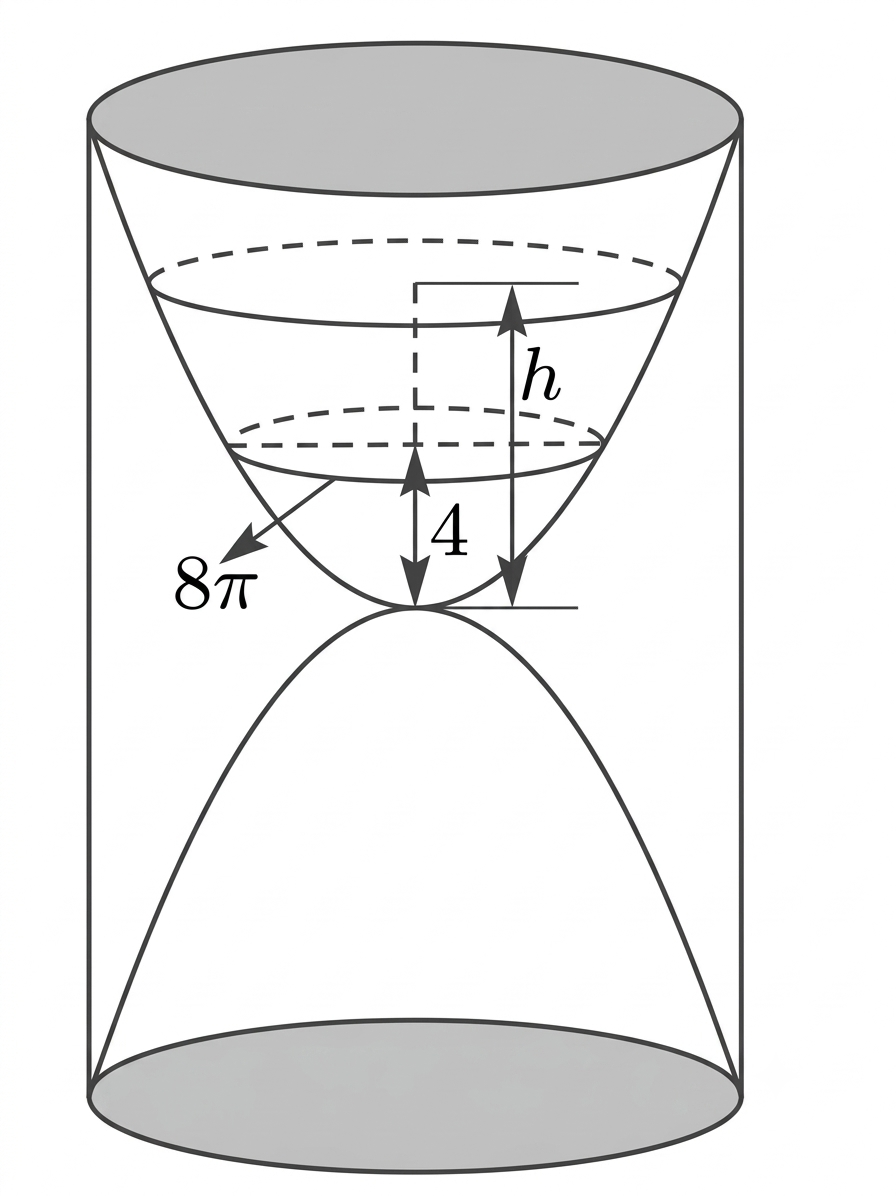
\includegraphics[width=0.2\textwidth]{../images/DHCat2.png}
\end{figure}
}


% --- CÂU 5 ---
\questionShortAnswer{0}{5}{Vệ tinh Van Allen Probes được phóng lên không gian để nghiên cứu các vành đai bức xạ bao quanh Trái Đất. Vệ tinh này bay theo một quỹ đạo có chu kỳ 10 giờ. Cứ mỗi vòng bay, vệ tinh lại xuyên qua vùng bức xạ mạnh và tích lũy thêm liều bức xạ. Biết rằng đơn vị của bức xạ là Gray (Gy), và khi tổng liều bức xạ chiếu vào vệ tinh đạt 1000 Gray, thì vệ tinh hỏng hoàn toàn. Khoảng cách từ tâm Trái Đất đến vệ tinh được mô hình hóa bằng hàm số \(R(T) = 7000 + 3000T\) km, trong đó \(T\) là thời gian tính bằng giờ, \(0 \leq T \leq 10\), kể từ đầu vòng bay. Công thức suất liều bức xạ, tức là lượng bức xạ vệ tinh nhận được trong 1 giờ, phụ thuộc vào khoảng cách \(R\) km từ vệ tinh tới tâm Trái Đất, là \(D(R) = 60\left(\dfrac{R}{25000}\right)^2\) milliGray/giờ. Biết rằng do tính đối xứng và chu kỳ của quỹ đạo bay, tổng liều bức xạ vệ tinh nhận được trong một vòng bay 10 giờ được tính bằng công thức \(L = 2\displaystyle\int_{0}^{5} D(R(T))dT\), và 1 Gray = 1000 milliGray. Tính số năm hoạt động của vệ tinh từ lúc bắt đầu hoạt động tới khi hỏng hoàn toàn. Không làm tròn các bước trung gian, chỉ làm tròn kết quả cuối cùng tới hai chữ số sau dấu phẩy, coi một năm có 365 ngày, mỗi ngày có 24 giờ.
}

% --- CÂU 6 ---
\questionShortAnswer{0}{6}{Tốc độ tăng trưởng chiều cao sau khi trồng (đơn vị: centimet/năm) của một loài cây lấy gỗ ở năm thứ \(t\) được cho bởi hàm số \(h'(t) = \log_{1,2}(20t + 1) + 30\). Từ năm thứ 20 đến năm thứ 30 sau khi trồng, cây cao thêm được bao nhiêu mét? (Làm tròn kết quả đến hàng phần trăm).
}

% --- CÂU 7 ---
\questionShortAnswer{0}{7}{Hai công ty, công ty A và công ty B, cùng ra mắt sản phẩm cạnh tranh thị trường mới vào cùng thời điểm. Thị phần được đo bằng số lượng khách hàng lũy kế.

Công ty A: Bắt đầu với 0 khách hàng. Trong giai đoạn đầu, chiến dịch marketing hiệu quả giúp tốc độ thu hút khách hàng mới của họ tăng dần theo thời gian, được mô tả bởi hàm \(f(t) = 2t + 7\) (nghìn khách hàng/tháng), với \(t\) là số tháng kể từ khi ra mắt.

Công ty B: Nhờ có uy tín từ trước, họ bắt đầu với 10 nghìn khách hàng đã đặt trước sẵn phẩm. Sau đó, họ duy trì một tốc độ thu hút khách hàng mới ổn định là 10 nghìn khách hàng/tháng.

Hỏi sau khoảng bao nhiêu tháng kể từ khi ra mắt, tổng số lượng khách hàng lũy kế của công ty A bằng tổng số lượng khách hàng lũy kế của công ty B (tính cả 10 nghìn khách hàng ban đầu)?
}

% --- CÂU 8 ---
\questionShortAnswer{0}{8}{Một bể cá hình trụ thủy tinh có bán kính đáy bằng 6 dm, chiều cao bằng 5 dm; bên trong bể cả người ta đặt một vật trang trí là khối nón đặc (đỉnh hình nón sẽ được bố trí với bơm nước cho bể cá), đáy hình nón có bán kính bằng 3 dm và có tâm trùng với đáy hình trụ, chiều cao hình nón bằng với chiều cao hình trụ. Người ta bơm nước vào bể với tốc độ 0,5 lít/phút; đến phút thứ 40 thì tốc độ dâng lên của nước là bao nhiêu cm/phút (làm tròn đến hàng phần trăm)?
\begin{figure}[H]
    \centering
    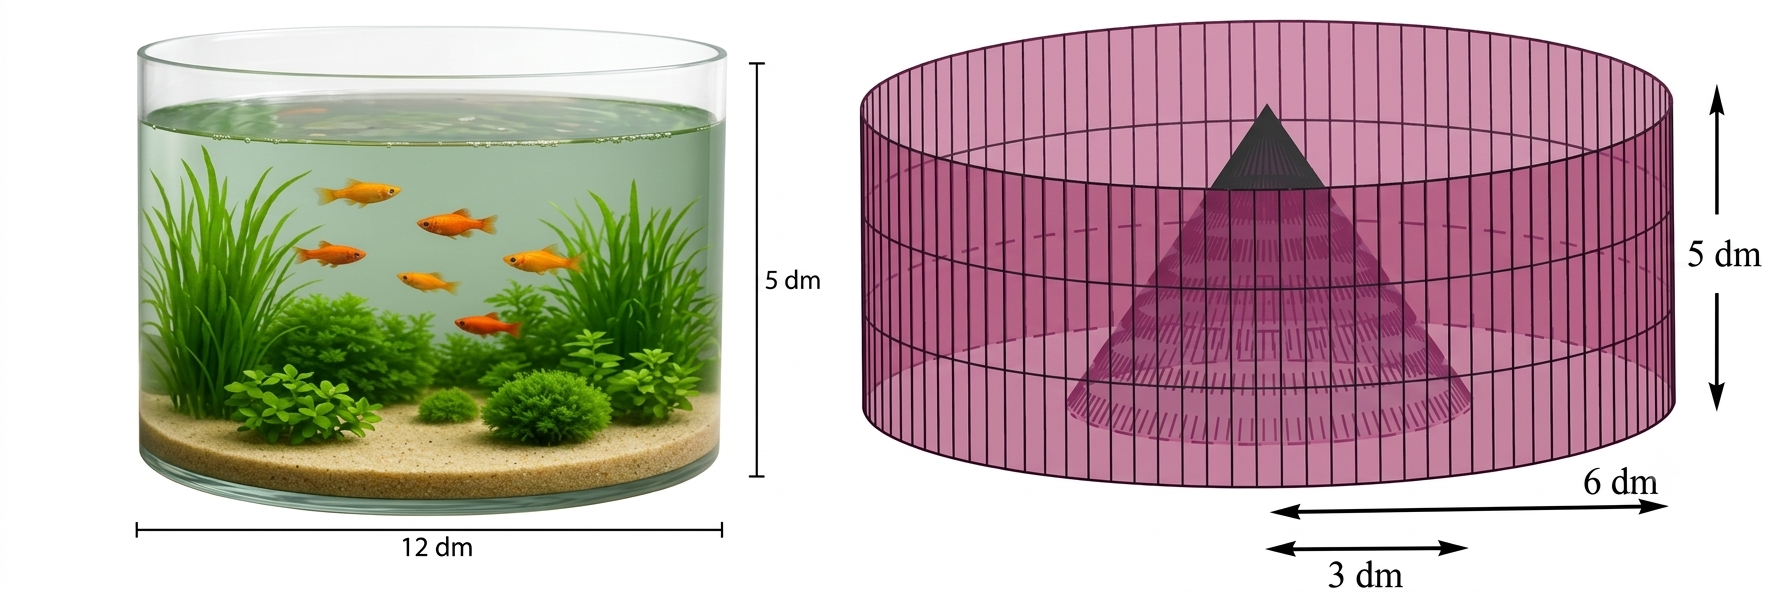
\includegraphics[width=0.6\textwidth]{../images/HoCa.png}
\end{figure}
}


\end{document}